
\chapter{Proposed Framework}
\label{capitulo4}
The framework was idealized to work and different scenarios, in the Section \ref{sub:1} is presented the proposal with one camera with the object calibration. In Section \ref{sub:2} is defined the problem with one camera, but using a known map with some metrics to estimate the position along the map. The Section \ref{sub:3} is defined the approach with multicameras and real-time processing. 



\section{Approach 1 - One camera with object calibration}\label{sub:1}

The first proposed is based on the approach of the authors of the paper \cite{8678911}, where it is necessary to calibrate the camera before start the object recognition and classification. This proposal were defined in six steps.

\begin{figure}[H]
\centering
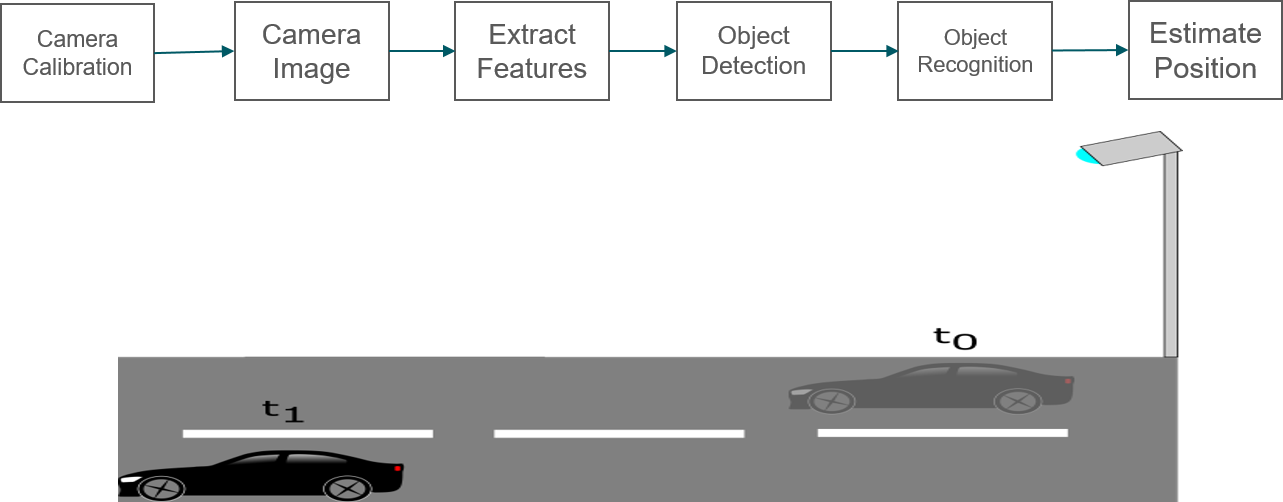
\includegraphics[width=\textwidth]{imagens/proposal1.png}
\caption{Proposal using only one camera with object calibration}
\label{fig:proposal1}
\end{figure}

\subsection{Camera Calibration}

For this task is necessary to reduce the distortion of the camera, the camera used on the tasks has a noise, for this approach is really recommend to perform this step. Following this requirement, a script in Python language with the OpenCV library based in \cite{zhu2020camera} was developed. Furthermore, with calibration you may also determine the relation between the camera’s natural units (pixels) and the real world units (for example millimeters).

Using the intrinsic parameters of the camera, using the in (\ref{eq:calibration}), one point is projected on the image plane. 

Where the 3D point ($X_w, Y_w, Z_w$) in the world coordinates to its projection ($u, v$) in the image image coordinates.


\begin{equation}
    \label{eq:calibration}
    \begin{bmatrix}
        u'
        \\v' 
        \\ z' 
        
        \end{bmatrix} = P \begin{bmatrix}
        X_w\\
        Y_w 
        \\ Z_w
        \\ 1
        
        \end{bmatrix}
\end{equation}

In \ref{eq:points}, $\mathbf{P}$ is a 3x4 projection matrix combined of two different parts, the intrinsic parameters of the camera ($\mathbf{K}$) and the extrinsic matrix ($[\mathbf{R}|t]$) that is based on the combination of 3x3 rotation matrix $\mathbf{R}$ and 3x1 translation $t$ vector. 

\begin{equation}
    \label{eq:points}
    P = \overbrace{\hbox{\boldsymbol{K}}}^{\hbox{Intrinsic Matrix}} x \overbrace{\hbox{[\boldsymbol{R}|t]}}^{\hbox{Extrinsic Matrix}}
\end{equation}

The intrisic matrix ($\mathbf{K}$) is an upper triangular matrix as shown in (\ref{eq:intrisic}). 

\begin{equation}
    \label{eq:intrisic}
\textbf{K} = \begin{bmatrix}
    f_x & \gamma  & c_x\\ 
    0 & f_y & c_y\\ 
    0 & 0 & 1
    \end{bmatrix}
\end{equation}

where, $f_x, f_y$ are the $x$ and $y$ focal lengths, $c_x, c_y$ are the $x$ and $y$ coordinates of the center in the image plane, $\gamma$ is the skew between the axes, in this master's thesis was defined equal to $0$.  

\subsection{Camera Image}

The image camera model depicted in Figure \ref{fig:image_formation} describes the mathematical relationship between the coordinates of a point in 3-dimension space and its projection onto
the image plane of a camera, where this aperture is described as a point and no lenses are used to focus light. This means that the model can only be used as a first order approximation of the mapping from a 3D scene to a 2D image \cite{forsyth2002computer}.




\begin{figure}[H]
\centering
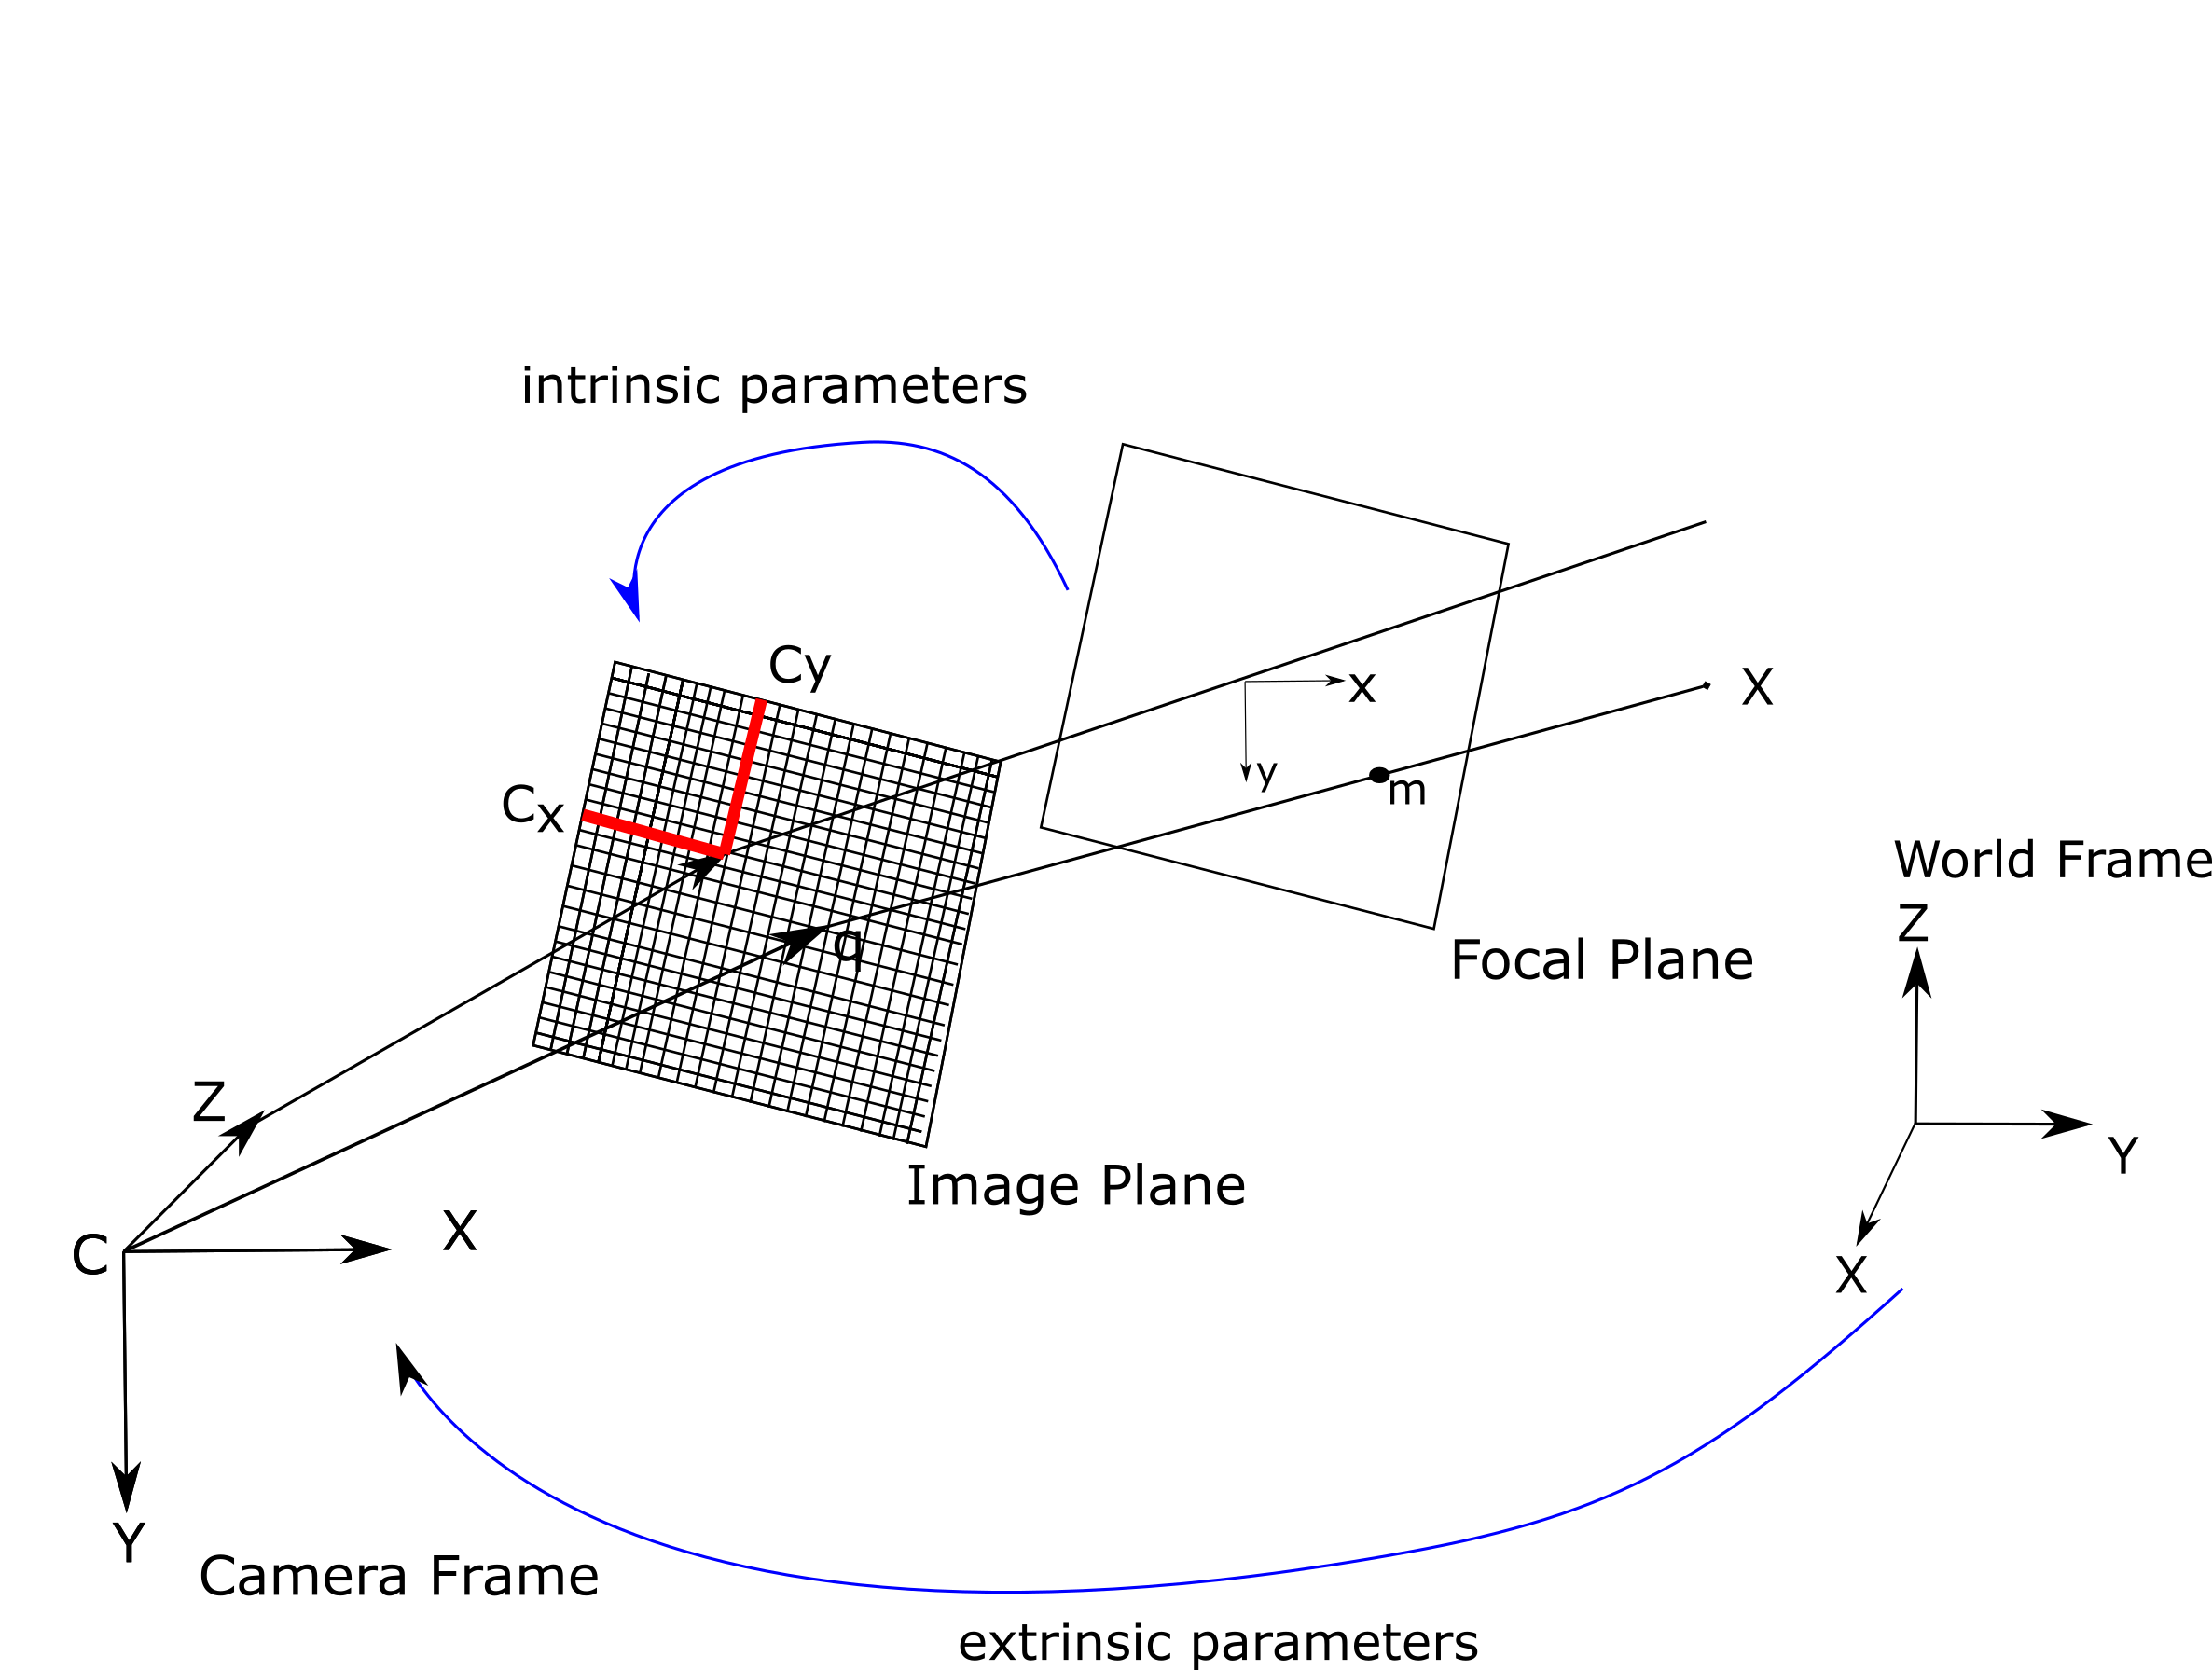
\includegraphics[width=\textwidth]{imagens/image_formation.png}
\caption{The camera model for image formation based on some metrics and known parameters}
\label{fig:image_formation}
\end{figure}

\subsection{Extract Features}

When it is necessary to work with variables that contains many contents, there is a necessity to improve this work and reduce the computer bottleneck during the process. In machine learning (ML), there are variables that are independents or some cases features on which the final output is done. And in other cases that numbers of these features increases it and reduce the ability to visualize the data. 

For example, the image resolution of the collected data for training part of the ML algorithm is $1392$ pixels in height and $512$ pixels in width, for the total $712,704$ pixels in total. Where each pixel has a single pixel-value associated with it, indicating the darkness or lightness of that pixel. The range of these numbers are between $0$ and $255$, and with this premise is necessary to determine which objects the image contains.

The task was performed by feature extraction which is a process to creating a new features from existing features, and with this allows to give more information and less redundancies \ref{wang2019data}.

A mathematical tool called Principal Component Analysis (PCA) was used in this step, and the PCA is used to decompose a multivariate dataset in a set of sucessive orthogonal components that explain a maximum amount of the variance \cite{pedregosa2011scikit}. In Figure \ref{fig:pca_step1} is shown how the technique works, the data is decomposed into perpendicular vector where the information is unrolled. And with more variance means more information of data.




\section{Approach 2 – One camera with known map}\label{sub:2}
\begin{figure}[H]
\centering
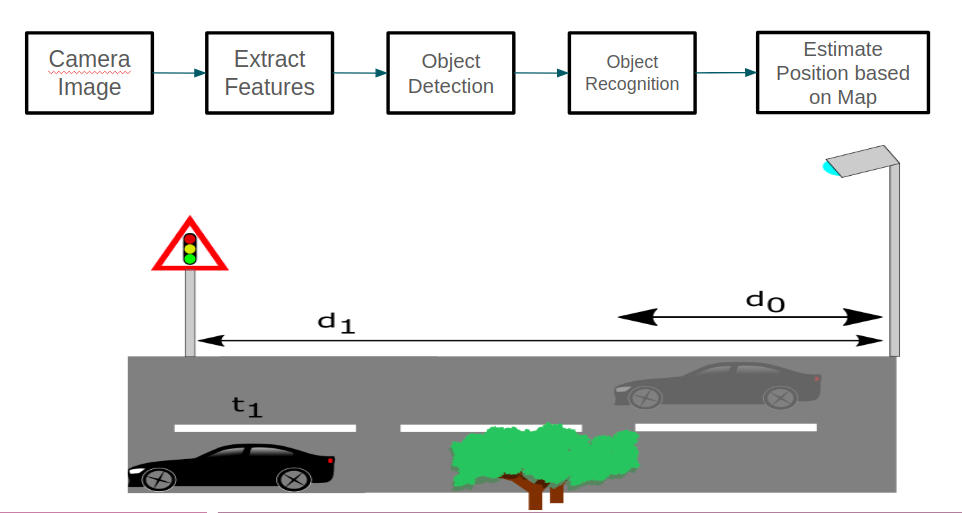
\includegraphics[width=\textwidth]{imagens/proposal2.png}
\caption{Approach using one camera with known map}
\label{fig:proposal2}
\end{figure}


\section{Approach 3 – Multicamera}\label{sub:3}
\begin{figure}[H]
\centering
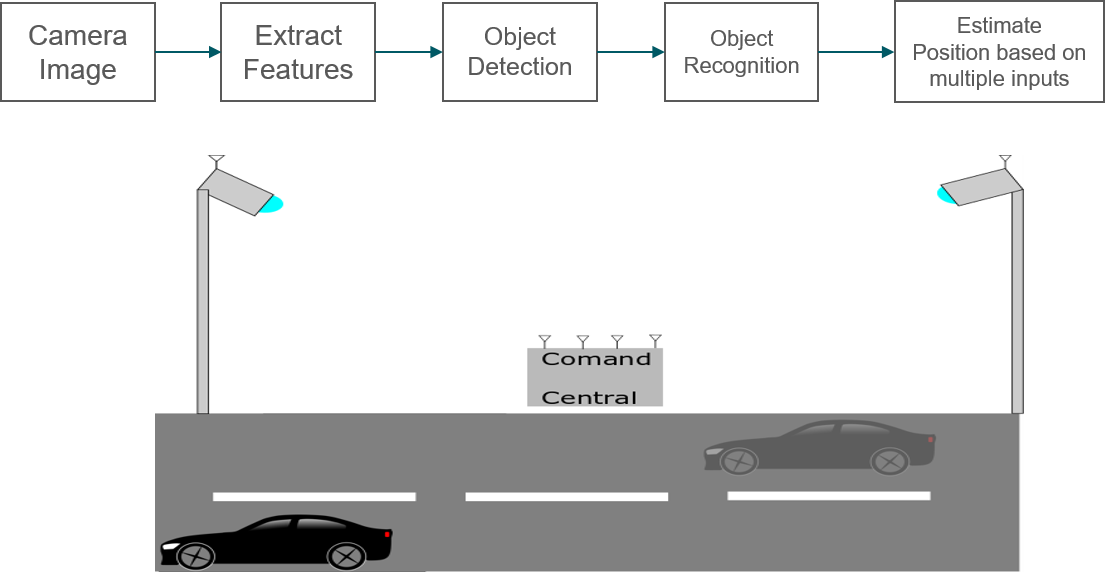
\includegraphics[width=\textwidth]{imagens/proposal3.png}
\caption{Approach using multicamera}
\label{fig:proposal3}
\end{figure}



\section{Inverse Perspective Mapping }
Inverse perspective mapping is a mathematical technique that remove the effects of distortion of a picture when transforming the perspective of the image to another perspective. In spite of disparity mapping, inverse perspective mapping method requires only one camera and this method cannot provide depth information directly ~\cite{Tuohy2010}.

Camera must be located in front of the car with an angle of \(\theta\) to down. Figure \ref{fig:ImageRelationSystem} shows the setup.

\begin{figure}[h]
\centering
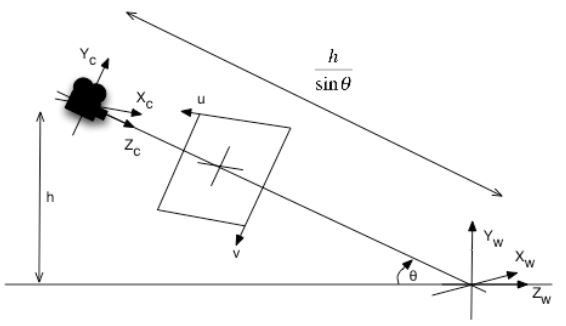
\includegraphics[scale=0.5]{imagens/Inverse Perspective Mapping.JPG}
\caption{Image coordinate system in relation to world coordinate
system.}
\label{fig:ImageRelationSystem}
\end{figure}
\par


This setup was selected based on solution of \cite{Wongsaree2018}, the mathematical background is to create top-down view, the surface road point is known as $(X_w,Y_w,Z_w)$
that projects to the image plane $(u,v)$ is a must. As disrupted in Figure \ref{fig:ImageRelationSystem}. For rotatation angle $(\theta)$, which is angle between camera and the surface, the IPM equation is based on \cite{7759904} and is shown is Equation \ref{eq:eq1}:

\begin{equation}
    (u,v,1)^T = K\cdot T \cdot K (X_w,Y_w, Z_w,1)^T
    \label{eq:eq1}
\end{equation}

where R is the rotation matrix given in the equation \ref{exp2}.
\begin{equation} \label{exp2}
R=
\begin{bmatrix}
1 & 0 & 0 & 0\\
0 & \cos{\theta} & -\sin{\theta} & 0\\
0 & \sin{\theta} & \cos{\theta} & 0\\
0 & 0 & 0 & 1
\end{bmatrix}
\end{equation}
\par

T is the translation matrix given in the equation \ref{exp3}. Where h means the height of the position of the camera.
\begin{equation} \label{exp3}
T=
\begin{bmatrix}
1 & 0 & 0 & 0\\
0 & 1 & 0 & 0\\
0 & 0 & 1 & \frac{-h}{\sin{\theta}}\\
0 & 0 & 0 & 1
\end{bmatrix}
\end{equation}


\par
K is the camera parameter matrix given in the Equation \ref{exp4}. Where $f$ is the focal length of the camera, $s$ is the skew parameter and $u_0, v_0$ are the center of the pixel of desired image size. 
\begin{equation} \label{exp4}
K =
\begin{bmatrix}
f & s & u_0 & 0\\
0 & f & v_0 & 0\\
0 & 0 & 1 & 0\\
\end{bmatrix}
\end{equation}

The Equation \ref{exp4} can be replaced using the real parameters of this test scenario and these parameters are $f = 2.92 mm, s=0, u_0=240, v_0=160$. Replacing the Equations \ref{exp2},\ref{exp3}, \ref{exp4} into the initial Equation \ref{eq:eq1}, achieving the new Equation \ref{eq:eq2}.

\begin{equation}
    \begin{bmatrix}
u\\ 
v\\ 
1
\end{bmatrix}
=\begin{bmatrix}
P_{11} & P_{12} & P_{13} & P_{14}\\ 
P_{21} & P_{22} & P_{23} & P_{24}\\ 
P_{31} & P_{32} & P_{33} & P_{34}
\end{bmatrix}
\begin{bmatrix}
X_w\\ 
Y_w\\ 
Z_w\\
1
\end{bmatrix}
\label{eq:eq2}
\end{equation}

where the matrix P was gotten from product between K, T, and R. As is only necessary to evaluate the position of the road, so the coordinate $Y_w$ can be equal to 0, so simplifying the Equation \ref{eq:eq2}, so it is given by Equation \ref{eq:eq3}.

\begin{equation}
    \label{eq:eq3}
    \begin{bmatrix}
u\\ 
v\\ 
1
\end{bmatrix}
=\begin{bmatrix}
P_{11} & P_{12}  & P_{14}\\ 
P_{21} & P_{22}  & P_{24}\\ 
P_{31} & P_{32}  & P_{34}
\end{bmatrix}
\begin{bmatrix}
X_w\\ 
Z_w\\
1
\end{bmatrix}
\end{equation}

Based on the Equations above, it is possible to infer the Equation \ref{eq:eq4} for compute the distance from the camera until the object. 

\begin{enumerate}
    \item Calculating average intensity in row direction from bottom row up to top row
    \item The average intensity of each row is compared with the threshold level (obtained from the experimental) which is 50. The starting position of an object is indicated if the average intensity in that row is greater than 50 and the order of that row is stored in a parameter p.
    \item The distance between object and vehicle is therefore calculated using a linear equation given in \ref{eq:eq4}.
\end{enumerate}

\begin{equation}
    \label{eq:eq4}
    d = ap+b
\end{equation}

where $d$ is distance between camera and object and vehicle in meter, $p$ is the order of the row that object is detected and $a, b$ are constants.

 
\section{Framework Architecture} 

\begin{figure}[H]
\centering
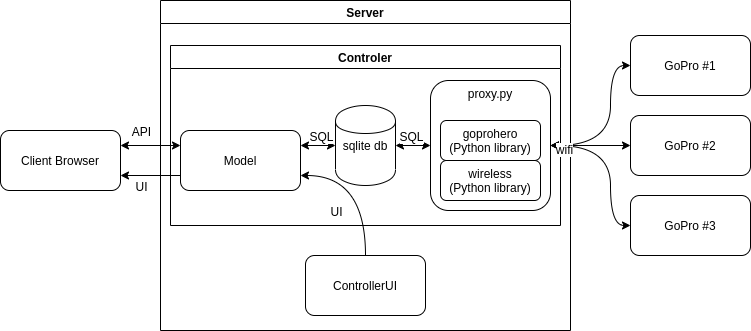
\includegraphics[scale=0.6]{imagens/diagram.png}
\caption{Architecture approach of framework}
\label{fig:framework}
\end{figure}

\begin{figure}[H]
\centering
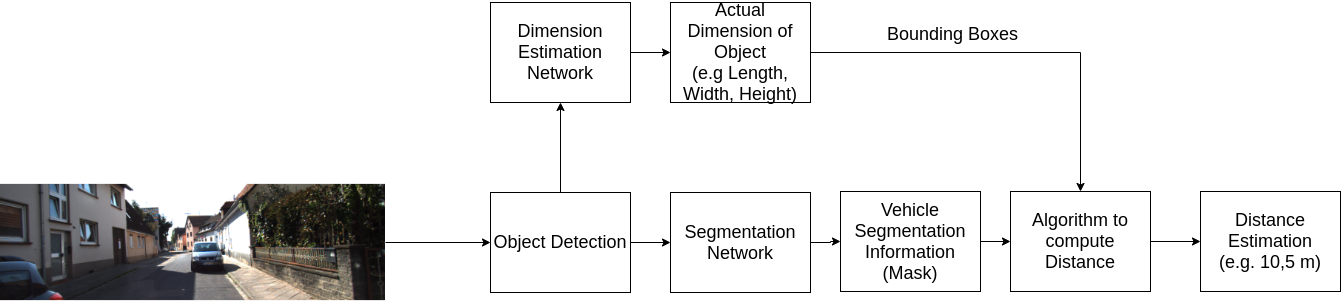
\includegraphics[width=\textwidth]{imagens/Network Behavior.png}
\caption{Architecture approach of framework}
\label{fig:networkBehavior}
\end{figure}